%% Template para dissertacao/tese na classe UFBAthesis
%% versao 1.0
%% (c) 2005 Paulo G. S. Fonseca
%% (c) 2012 Antonio Terceiro
%% (c) 2014 Christina von Flach
%% www.dcc.ufba.br/~flach/ufbathesis

%% Carrega a classe ufbathesis
%% Opcoes: * Idiomas
%%           pt   - portugues (padrao)
%%           en   - ingles
%%         * Tipo do Texto
%%           bsc  - para monografias de graduacao
%%           msc  - para dissertacoes de mestrado (padrao)
%%           qual - exame de qualificacao de mestrado
%%           prop - exame de qualificacao de doutorado
%%           phd  - para teses de doutorado
%%         * Media
%%           scr  - para versao eletronica (PDF) / consulte o guia do usuario
%%         * Estilo
%%           classic - estilo original a la TAOCP (deprecated) - apesar de deprecated, manter esse.
%%           std     - novo estilo a la CUP (padrao)
%%         * Paginacao
%%           oneside - para impressao em face unica
%%           twoside - para impressao em frente e verso (padrao)

% Atencao: Manter 'classic' na declaracao abaixo:
\documentclass[qual, classic, a4paper]{ufbathesis}

%% Preambulo:
\usepackage[utf8]{inputenc}
\usepackage{graphicx}
\usepackage{lipsum}
\usepackage{hyphenat}
\usepackage[usenames, dvipsnames, table]{xcolor}
\usepackage{booktabs}
\usepackage{pifont}
\usepackage{multirow}
\usepackage{listings} 
%\usepackage{colortbl}
\usepackage{xfrac}
\usepackage[FIGTOPCAP]{subfigure}
\usepackage[printonlyused, withpage]{acronym}
\usepackage{multirow}
\usepackage{color, colortbl}
\usepackage{enumitem}
\usepackage{gensymb}
\usepackage{subfigure}
%https://tex.stackexchange.com/questions/163768/write-pseudo-code-in-latex 
\usepackage{amsmath}
%\usepackage{algorithmic} %https://tex.stackexchange.com/questions/28627/how-to-install-the-algorithms-package/28629
%\usepackage{algorithm}
%\usepackage[noend]{algpseudocode}
\usepackage[]{algorithm2e} 	%http://linorg.usp.br/CTAN/macros/latex/contrib/algorithm2e/doc/algorithm2e.pdf
							%https://en.wikibooks.org/wiki/LaTeX/Algorithms#Typesetting_using_the_algorithmic_package
%\usepackage{caption, subcaption}
   %\captionsetup[sub]{labelformat=simple}
    %\renewcommand{\thesubfigure}{(\alph{subfigure})} % Style: 1(a), 1(b)

%\usepackage{tikz}

%\usetikzlibrary{arrows,positioning,shapes}

%\usepackage[colorlinks,citecolor=blue]{hyperref}

\graphicspath{{./figuras/}}

%https://tex.stackexchange.com/questions/163768/write-pseudo-code-in-latex
\makeatletter
\def\BState{\State\hskip-\ALG@thistlm}
\makeatother

%\definecolor{Gray}{gray}{0.9}

% Universidade
\university{Universidade Federal da Bahia}

% Endereco (cidade)
\address{Salvador}

% Instituto ou Centro Academico
\institute{Instituto de Matem\'{a}tica}

% Nome da biblioteca - usado na ficha catalografica
\library{Biblioteca Reitor Mac\^{e}do Costa}

% Programa de pos-graduacao
\program{Programa de P\'{o}s-Gradua\c{c}\~{a}o em Ci\^{e}ncia da Computa\c{c}\~{a}o}

% Area de titulacao
\majorfield{Ci\^{e}ncia da Computa\c{c}\~{a}o}

% Titulo da dissertacao
\title{Uma Proposta de Simula\c{c}\~{a}o Computacional 3D para Pintura Hidrogr\'{a}fica}

% Data da defesa
% e.g. \date{19 de fevereiro de 2013}
\date{10 de julho de 2018}
% e.g. \defenseyear{2013}
\defenseyear{2018}

% Autor
% e.g. \author{Jose da Silva}
\author{Leonardo Thomas Torres Santos}

% Orientador(a)
% Opcao: [f] - para orientador do sexo feminino
% e.g. \adviser[f]{Profa. Dra. Maria Santos}
\adviser{Karl Philips Apaza Ag\"{u}ero}

% Orientador(a)
% Opcao: [f] - para orientador do sexo feminino
% e.g. \coadviser{Prof. Dr. Pedro Pedreira}
% Comente se nao ha co-orientador
% \coadviser{Nome Completo do CO-ORIENTADOR}

%% Inicio do documento
\begin{document}

\pgcompfrontpage

%% Parte pre-textual
\frontmatter

\pgcomppresentationpage

%%%%%%%%%%%%%%%%%%%%%
% Resumo em Portugues
%%%%%%%%%%%%%%%%%%%%%
\resumo

A Pintura Hidrográfica, \textit{Water Transfer Printing} ou \textit{Hydrographics} é uma técnica viável para colorir objetos criados em impressoras 3D. Porém, neste tipo de pintura há uma complexa interação entre um filme e um objeto impresso em 3D, na qual a imagem contida no filme deve aderir ao objeto. Este processo está sujeito a incertezas sobre como o filme se deformará para aderir ao objeto impresso em 3D e transferir a imagem para a superfície do objeto, conferindo-lhe um acabamento resultado de um mapeamento de uma imagem 2D em um modelo real 3D.

Diante destas dificuldades, será apresentada uma proposta de simulação computacional 3D para a técnica de pintura hidrográfica. Com base na interação física entre os corpos envolvidos neste fenômeno, será proposta uma simulação computacional 3D que mostre o que ocorre durante a pintura hidrográfica. Desta forma, será dado ao usuário um suporte ao usuário para antever o processo da pintura em formas mais complexas, que necessitem de alinhamentos com a imagem transferida ao objeto. Além disso, o trabalho também busca simular o fenômeno físico da pintura hidrográfica em tempo real, fazendo uma avaliação da utilização dos recursos computacionais da \acs{GPU} (\acl{GPU}) empregados nesta simulação.
 
% Palavras-chave do resumo em Português
\begin{keywords}
Impressão 3D, pintura hidrográfica, simulação baseada em física, renderização em tempo real, mapeamento de texturas 
\end{keywords}


%%%%%%%%%%%%%%%%%%%
% Resumo em Ingles
%%%%%%%%%%%%%%%%%%%

\abstract

Hydrographic printing, Water Transfer Printing or Hydrographics is a viable technique for coloring objects created with 3D printers. However, in this type of painting there is a complex interaction between a film and a 3D printed object, in wich the image contained in the film must adhere over the object. This process is subjected to several uncertainties about how the film will deform to adhere over the 3D object and transfer the image to the surface of the object, giving it a finish resulting from a mapping of a 2D image into a real 3D model.

Faced with these difficulties, a 3D computational simulation proposal will be presented for the hydrographic printing technique. Based on the physical interaction between the bodies involved in this phenomenon, it will be proposed a 3D computer simulation that shows what happens during hydrographic printing. In this way, the user will be given a support to preview the painting process in more complex shapes, which require alignments with the image transferred to the object. Futhermore, the work also aims to simulate the physical phenomenon of hydrographic printing in real time, making an evaluation of the use of the computational resources of the \ac{GPU} used in this simulation.

% Palavras-chave do resumo em Ingles
\begin{keywords}
3D printing, hydrographic printing, physically-based animation, real-time rendering, texture mapping
\end{keywords}


%%%%%%%%%%%%%%%%%%%
% Sumario / Indice
%%%%%%%%%%%%%%%%%%%

% Comente para ocultar
\tableofcontents

% Lista de figuras
% Comente para ocultar
\listoffigures

% Lista de tabelas
% Comente para ocultar
\listoftables

\chapter*{Lista de Siglas}

% Sintaxe da lista de acordo com a documentação do pacote `acronym'
% documentação: http://mirror.unl.edu/ctan/macros/latex/contrib/acronym/acronym.pdf
\begin{acronym}[PGCOMP]
     \acro{API}[API]{\textit{Application Programming Interface}}
     \acro{CPU}[CPU]{\textit{Central Processing Unit}}
     \acro{CNPq}[CNPq]{Conselho Nacional de Desenvolvimento Científico e Tecnológico}
     \acro{FPS}[FPS]{Frames por Segundo}
     \acro{GPU}[GPU]{\textit{Graphics Processing Unit}}
     \acro{MAE}[MAE]{Museu de Arqueologia e Etnologia da UFBA}
     \acro{MEF}[MEF]{Método dos Elementos Finitos}
     \acro{OpenGL}[OpenGL]{\textit{Open Graphics Library}}
     \acro{PBD}[PBD]{\textit{Position-based Dynamics}}
     \acro{PGCOMP}[PGCOMP]{Programa de Pós-Graduação em Ciência da Computação}
     \acro{WTP}[WTP]{\textit{Water Transfer Printing}}
\end{acronym}

%% Parte textual
\mainmatter

% Eh aconselhavel criar cada capitulo em um arquivo separado, digamos
% "capitulo1.tex", "capitulo2.tex", ... "capituloN.tex" e depois
% inclui-los com:
% \xchapter{Introdu\c{c}\~{a}o}{Este eh o primeiro cap\'{\i}tulo, onde eu conto toda a historia deste trabalho, o problema, a solu\c{c}\~{a}o, etc.}

Texto da introdução com a contextualização, o marco teórico e a formulação de hipóteses.

% É recomendável utilizar `\acresetall' no início de cada capítulo para reiníciar o contator de referências às siglas.
\acresetall 

\section{Se\c{c}\~{a}o}
Trabalho do  \ac{PGCOMP}. Bolsa do \ac{CNPq}.

\begin{figure}[h]
    Figure
    \caption{As siglas também funcionam nas legendas, seja na forma de sigla \ac{CNPq}, seja na forma completa \acf{PGCOMP}.}
\end{figure}


\subsection{Uma Subse\c{c}\~{a}o}
\acresetall
Texto para mostrar como o \verb|\acresetall| funciona \ac{CNPq}, \ac{PGCOMP}. Ele reseta os contadoes e faz a sigla aparecer na forma estendida novamente.

\subsection{Outra Subse\c{c}\~{a}o}

Texto  \acf{CNPq}, \acf{PGCOMP}.

% \xchapter{Revis\~{a}o Bibliogr\'{a}fica}{Neste cap\'{\i}tulo eu apresento todo o material que eu estudei durante a elabora\c{c}\~{a}o do trabalho.}

Texto da introdução com a contextualização, o marco teórico e a formulação de hipóteses.

Exemplos de cita\c{c}\~{o}es no cap\'{i}tulo 2
Livro \cite{demeyer2008} e  livro \cite{raymond1999}. Tamb\'{e}m o artigo \cite{zhang2015}, tem também o \cite{panozzo2015}


% ...
% \include{capituloN}
%
% Importante: 
% Use \xchapter{}{} ao inves de \chapter{}; se nao quiser colocar texto antes do inicio do capitulo, use \xchapter{texto}{}.

\xchapter{Introdu\c{c}\~{a}o}{Este eh o primeiro cap\'{\i}tulo, onde eu conto toda a historia deste trabalho, o problema, a solu\c{c}\~{a}o, etc.}

Texto da introdução com a contextualização, o marco teórico e a formulação de hipóteses.

% É recomendável utilizar `\acresetall' no início de cada capítulo para reiníciar o contator de referências às siglas.
\acresetall 

\section{Se\c{c}\~{a}o}
Trabalho do  \ac{PGCOMP}. Bolsa do \ac{CNPq}.

\begin{figure}[h]
    Figure
    \caption{As siglas também funcionam nas legendas, seja na forma de sigla \ac{CNPq}, seja na forma completa \acf{PGCOMP}.}
\end{figure}


\subsection{Uma Subse\c{c}\~{a}o}
\acresetall
Texto para mostrar como o \verb|\acresetall| funciona \ac{CNPq}, \ac{PGCOMP}. Ele reseta os contadoes e faz a sigla aparecer na forma estendida novamente.

\subsection{Outra Subse\c{c}\~{a}o}

Texto  \acf{CNPq}, \acf{PGCOMP}.
%introducao

\xchapter{Revis\~{a}o Bibliogr\'{a}fica}{Neste cap\'{\i}tulo eu apresento todo o material que eu estudei durante a elabora\c{c}\~{a}o do trabalho.}

Texto da introdução com a contextualização, o marco teórico e a formulação de hipóteses.

Exemplos de cita\c{c}\~{o}es no cap\'{i}tulo 2
Livro \cite{demeyer2008} e  livro \cite{raymond1999}. Tamb\'{e}m o artigo \cite{zhang2015}, tem também o \cite{panozzo2015}

%fundamentacao

\xchapter{Defini\c{c}\~{a}o da proposta}{Será feita uma descrição da proposta, detalhamento dos recursos necessários, primeiros resultados, cronograma }

\acresetall

\section{Proposta}

A proposta para realização deste projeto de pesquisa divide-se em três grandes frentes de trabalho:

\begin{itemize}
\item Realização do experimento físico
\item Implementação de uma simulação computacional 
\item Elaboração da dissertação e artigos
\end{itemize}

Estas três frentes são executadas em paralelo, incrementalmente, partindo de um estágio menos elaborado (com protótipos) e progressivamente chegando ao estágio mais elaborado (refinamentos do protótipo inicial), até o fim do trabalho.

\subsection{Realização do experimento físico}

Para realização do experimento físico, foram empregados os materiais básicos para a impressão hidrográfica descritos no \ref{apendice1:material}.

Um experimento preliminar foi realizado com uma peça de prova impressa em 3D e uma película hidrográfica com uma estampa de padronagem similar à fibra de carbono. A peça de prova escolhida foi um modelo 3D de um artefato cultural com formato de tartaruga, que encontra-se no acervo do Museu de Arqueologia e Etnologia da UFBA. Isto porque é possível que os resultados deste projeto sejam aproveitados para colorir outras peças do acervo, que atualmente está sendo submetido a um processo de reconstrução 3D.

A figura \ref{fig:experimento1} é uma foto do aspecto final da peça de prova utilizada no experimento preliminar.

\begin{figure}
\begin{center} 
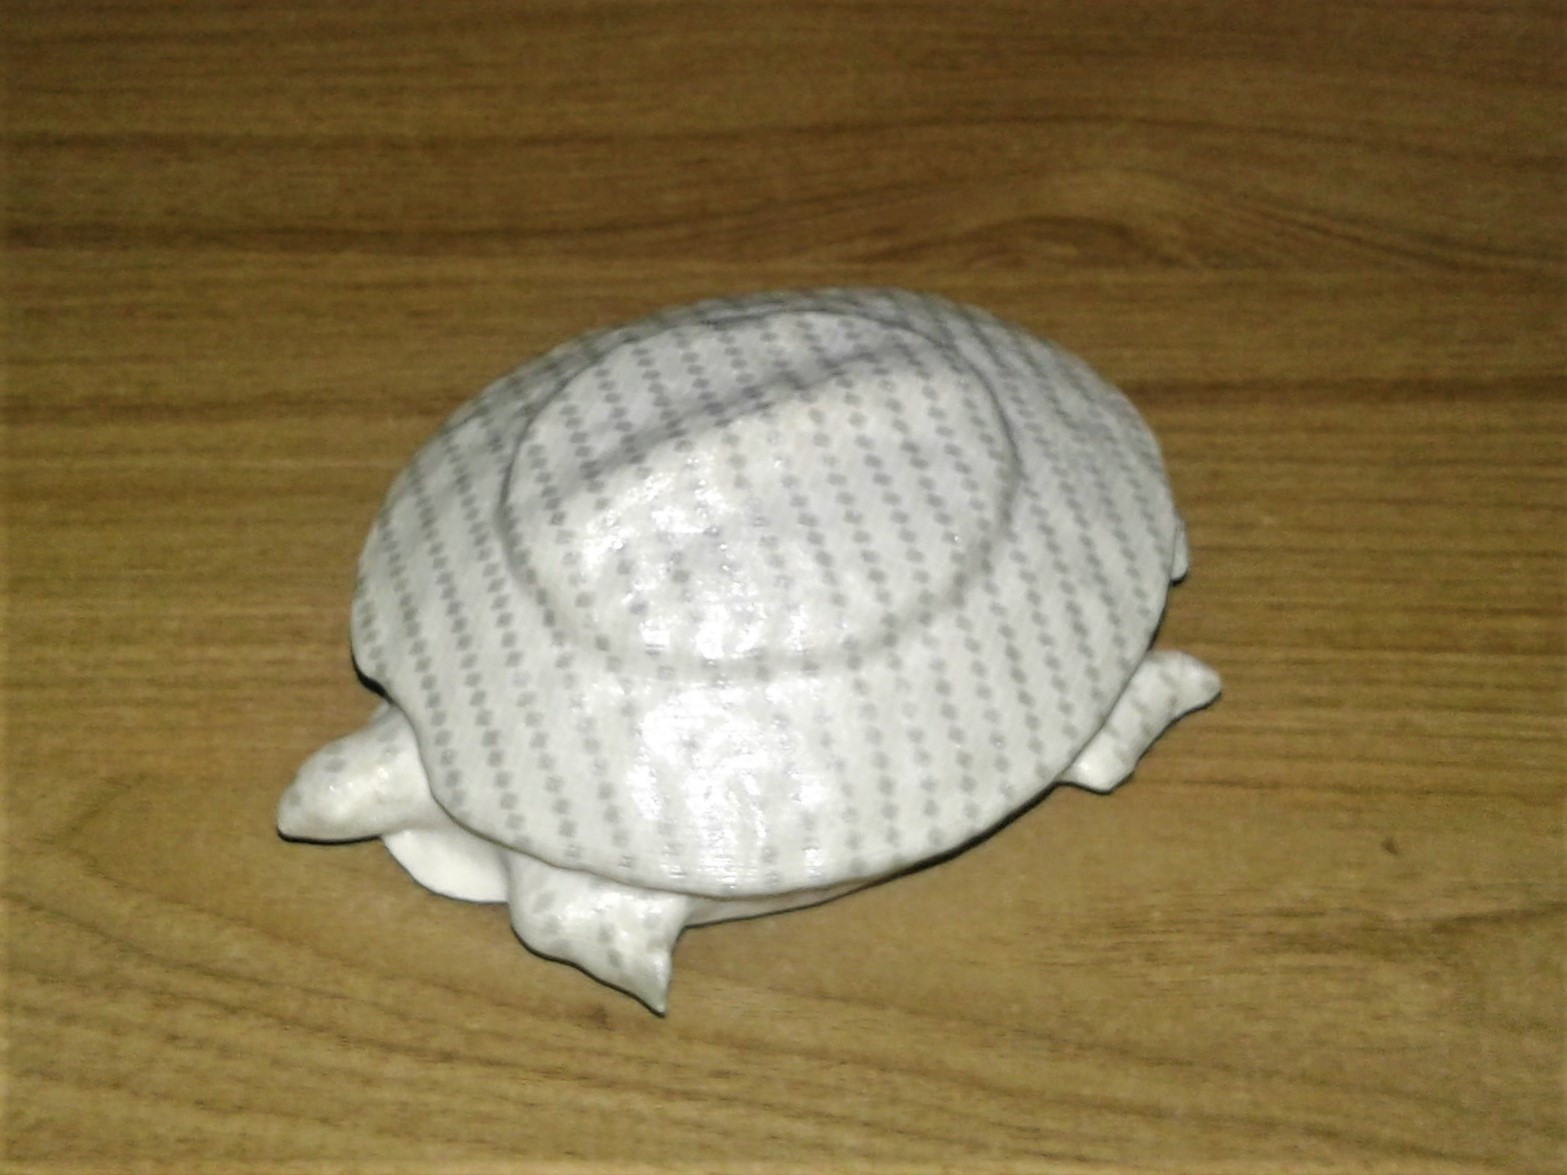
\includegraphics[scale=0.15]{experimento1.jpg}
\caption{Experimento preliminar.}
\label{fig:experimento1}
\end{center} 
\end{figure}

A partir deste experimento preliminar, foi possível realizar anotações relevantes sobre o funcionamento da técnica. Estas anotações, junto às observações feitas em trabalhos anteriores foram levadas em consideração para a implementação da primeira simulação em software.

Posteriormente, para a criação de películas com estampas customizadas, será preciso realizar impressões em uma impressora com tinta pigmentada em um filme para pintura hidrográfica apropriado. A tinta pigmentada, por apresentar resistência à água, oferece melhor fixação para o propósito da pintura hidrográfica. Nesta etapa do trabalho, está sendo avaliado se será utilizado um serviço de impressão com tinta pigmento contratando uma gráfica ou se será adquirida uma impressora específica para este fim.

\subsection{Implementação da simulação computacional}

Foi desenvolvido um software em C++ com OpenGL 4.3 e uso eficiente da GPU para renderização da simulação, que ocorre em tempo real. 

A simulação computacional da pintura hidrográfica partiu da hipótese de que o comportamento do filme que flutua na superfície da água seria semelhante ao comportamento de uma malha deformável de pontos 2D. Quando colide com um corpo rígido em velocidade constante, a malha sofre uma deformação conforme a forma e o movimento do objeto que se desloca verticalmente, de cima para baixo, paralelo ao eixo Y. 

Para efeito de simplificação dos cálculos para a verificação da colisão, o corpo rígido escolhido para a primeira simulação foi uma esfera.

O software de simulação recebe os parâmetros para criação da malha, que inicialmente são as quantidades de pontos na sua largura L e comprimento C. Inicialmente não é especificado um parâmetro para expressar a espessura da malha. No entanto, esta informação é necessária e encontra-se fixa na simulação inicial implementada. Também é passado para o programa principal um parâmetro referente à distância entre os pontos, o grau de rigidez (que determinará o quanto a malha poderá esticar), e a textura que a malha assumirá. 

Nesta simulação preliminar, foram determinadas duas opções de textura: um padrão xadrez e um mapa-múndi. A função de mapeamento da textura para a malha é definida em através da fração da distância entre os vértices (dos triângulos que compõem a malha) e a dimensão total da malha. Os vértices da malha recebem, além das suas coordenadas e das suas normais, qual a coordenada de textura mapeada. A aplicação da textura ocorre ainda quando a malha está plana. Quando a forma da malha é alterada, como os pontos já estão vinculados às coordenadas de textura, o desenho é igualmente deformado, representando a distorção sofrida pela película da hidropintura ao aderir a um substrato.

\begin{figure}
\begin{center} 
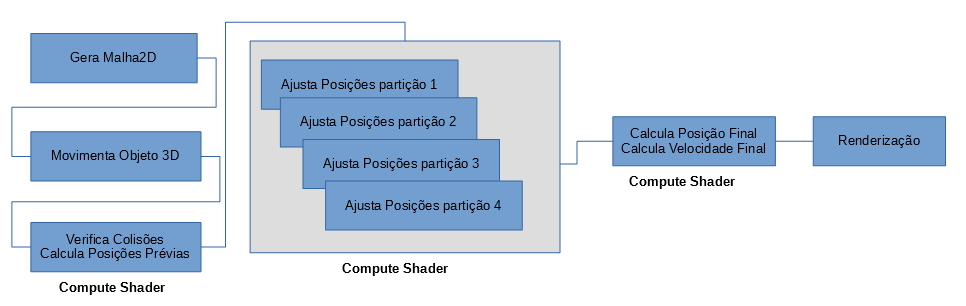
\includegraphics[scale=0.6]{diagrama_implementacao.png}
\caption{Representação das etapas do algoritmo implementado.}
\label{fig:diagrama_implementacao}
\end{center} 
\end{figure}

Para simular a deformação da malha, foi assumido que os pontos do filme que colidiram com o objeto seguirão a mesma velocidade vertical deste corpo. Isto seria suficiente para representar a adesão da película ao corpo em movimento. 

O processo de verificação da colisão da esfera com a malha 2D foi implementado através de um \textit{compute shader}. Para este \textit{compute shader}, foram passados: posição, raio e velocidade da esfera, espessura do filme, um vetor com as posições de todos os vértices compõem a malha 2D. Este vetor é indexado através de recursos próprios do OpenGL, que permitem sistematizar a execução das instâncias dos \textit{compute shaders}, criando identificadores únicos para cada instância. Na implementação feita, \textit{compute shaders} são disparados simultaneamente através de grupos de trabalho determinados pelas dimensões L e C da malha 2D. Cada grupo de trabalho, por sua vez, subdivide-se em dimensões X e Y expressas na propriedade \textit{local size}, definida internamente no \textit{compute shader}. O dimensionamento do \textit{local size} foi afixado com o valor constante de 4 x 4, o que representou na prática um azulejamento da malha. Sendo assim, uma malha 2D de dimensões 64 x 32 pontos foi segmentada em azulejos 4 x 4, representando um total de 128 \textit{compute shaders} processados simultaneamente. Cada instância deste \textit{compute shader} verifica a distância entre um ponto do plano e o raio da esfera. Caso esta distância seja menor do que uma distância mínima estabelecida (considerando-se também a espessura da película), então houve a colisão. Neste caso, o ponto do plano seguirá o mesmo movimento no eixo Y imposto pela esfera. 

Após verificação da colisão, os demais pontos do filme, que ainda não aderiram ao objeto, são puxados pelo movimento do objeto. Estes pontos seguirão com uma velocidade que será uma composição da velocidade do objeto com a velocidade imposta pelas partículas vizinhas (através do cálculo das restrições). Na simulação preliminar, estes pontos da malha são mantidos equidistantes com a técnica \acs{PBD} (\acl{PBD}). As partículas da malha são associadas duas a duas a uma restrição de distância. A cada intervalo de tempo, as posições das partículas são recalculadas, mantendo a restrição de distância. O recálculo da velocidade é necessário pois dá o efeito realista de movimentação da malha, fazendo com que de maneira natural a película abrace o objeto, tal qual ocorre no experimento físico.

A paralelização do algoritmo com \acs{PBD} para aplicação das restrições de distância se deu com base no estudo apresentado em \cite{fratarcangeli2013gpu}. Para o cálculo paralelizado seja possível, é necessário implementar uma forma de indexar os vértices da malha, agrupando os pares de vértices que podem ser calculados independente dos outros. Esta técnica pode ser comparada ao cálculo da coloração de um grafo. Com isto, é possível tratar a atualização de malhas que possuam partículas que tenham interferências entre si.

Na implementação, \textit{design} das restrições seguiu uma topologia na qual cada ponto da malha ficou com uma vizinhança dos pontos situados acima, abaixo, à sua direita, ou à sua esquerda. Sendo assim, exceto pelos pontos que situam-se nas bordas da malha - que possuem 2 ou 3 vizinhos - cada ponto possui 4 vizinhos. O cálculo da coloração do grafo determinou que nesta topologia, podem ser formados 4 partições da malha (representadas pelas cores), de forma que cada partição deve ser processada sequencialmente, sem interferir nas demais. A figura \ref{fig:topologia1} mostra a configuração das restrições e as cores representam as partições determinadas na implementação desta estrutura.

A figura \ref{fig:diagrama_implementacao} traz um diagrama que representa as etapas mais importantes da implementação feita.

\begin{figure}
\begin{center} 
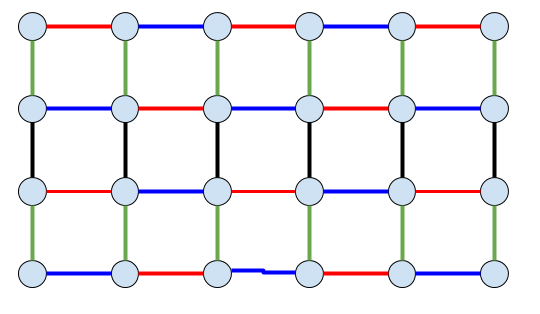
\includegraphics[scale=0.5]{paralelizacao.png}
\caption{Representação das restrições de distância como sendo as linhas que ligam os vértices da malha 2D. As cores representam as partições do conjunto de vértices, que deve ser processado sequencialmente pelo \textit{compute shader}.}
\label{fig:topologia1}
\end{center} 
\end{figure}

No algoritmo implementado, recálculo das velocidades e posições finais através (após o cálculo particionado das restrições) também foi realizado com o uso de \textit{compute shaders}, aproveitando a mesma lógica de indexação e azulejamento empregado no cálculo das colisões. Com isto, foi possível realizar uma simulação que proporcionasse a atualização final das posições com mais fluidez.

\subsubsection{Resultados iniciais}

A simulação foi executada em um ambiente compatível com:

\begin{itemize}
\item Processador Intel Core i5 7th Gen 7200U 2.5HGHz
\item Windows 10
\item Opengl 4.3 ou superior
\item Placa gráfica NVDIA GeoForce 940MX com 2GB de memória RAM dedicada
\item 8GB de memória RAM DDR4
\item 1GB de disco rígido
\end{itemize}

O software implementado possui as seguintes características:

\begin{itemize}
\item Simula através de uma animação computacional em tempo real a impressão hidrográfica de um dos padrões (xadrez ou mapa-múndi) em uma esfera.
\item Permite verificar a distorção do filme em 3 câmeras diferentes.
\item Permite iniciar e parar o movimento da impressão hidrográfica.
\item Permite girar a cena.
\end{itemize}

A principal parte do algoritmo da simulação está implementada em um laço, muito semelhante a uma animação baseada em física com a estrutura da integração Euleriana. A principal distinção entre esta simulação e a integração Euleriana é que esta basea-se no cálculo das posições. Como é sabido, pela técnica de \acs{PBD} o cálculo de posições de uma malha que sofreu uma colisão é resolvido através de um sistema de equações formado pelo conjunto de restrições com cardinalidade conhecida e um conjunto de posições com cardinalidade desconhecida que é dado como o cálculo de um sistema não linear. A resolução deste sistema é resolvida com iterações, através aproximação que leva ao método de Gauss-Siedel.

A próxima etapa da simulação é calcular a posição dos pontos que colidiram. Isto é feito em duas situações distintas: no primeiro caso, o vértice que colidiu adera à superfície do objeto, assumindo a mesma velocidade e posição do objeto. Em uma segunda situação, o após a primeira colisão, haverá uma propagação do movimento para os pontos que ainda não colidiram. Esta propagação será imediatamente percebida nos elementos vizinhos aos que colidiram. Para os elementos mais distantes da colisão, esta propagação será mais lenta. Esta etapa também é executada por um \textit{compute shader}, que dispara em paralelo o cálculo das restrições de toda a malha. 

A sequência de imagens na figura \ref{fig:simulacao} foi capturada da simulação da pintura obtida com esta implementação preliminar com a textura do mapa-múndi e uma malha de dimensões 32 x 64 pontos, totalizando 2048 pontos. 

\begin{figure}
\begin{center} 
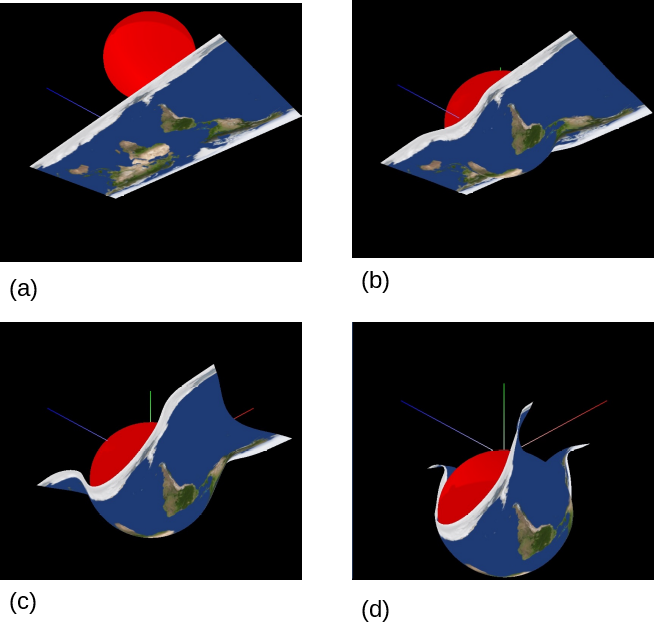
\includegraphics[scale=0.5]{simulacao_completa.png}
\caption{\textbf{(a)} Início da simulação. \textbf{(b)} Esfera tocando a película. \textbf{(c)} O objeto continua a se movimentar esticando a película. \textbf{(d)} A película segue o movimento aderindo ao objeto. }
\label{fig:simulacao}
\end{center} 
\end{figure}

A verificação da eficácia da técnica será feita comparando-se os resultados de pinturas com uma pintura guiada a partir da simulação hidrográfica computacional. A simulação será considerada bem-sucedida na medida em que conseguir reproduzir fidedignamente uma pintura física. Também se busca uma simulação com uma boa taxa de \acs{FPS} (\acl{FPS}). Na etapa de avaliação de resultados, serão testados objetos com superfícies arbitrárias e serão feitas medições com algumas variações em função da quantidade de pontos calculados na cena e da quantidade de iterações feitas na simulação.

\subsection{Elaboração da dissertação e artigos}

A elaboração da dissertação partirá da consolidação do levantamento bibliográfico, do refinamento das anotações realizadas em todas etapas da experimentação, análise de dados, bem como o aproveitamento de parte da estrutura e do texto da qualificação.

A partir da etapa de qualificação, serão gerados dois artigos: o primeiro com base na proposta e resultados iniciais da qualificação, e o segundo com a pesquisa e resultados finais gerados até a conclusão do mestrado.

A estratégia para submissão de artigos se dará selecionando os congressos e revistas nacionais e internacionais relevantes na área da computação gráfica, priorizando os que possuam melhor qualificação.

\section{Cronograma}

A tabela \ref{tab:cronograma} lista as atividades que serão feitas até a conclusão do mestrado.

\begin{table}[htbp]
\caption{Cronograma das atividades do mestrado.}

\begin{center}
\begin{tabular}{|*{13}{c|}}
\hline
\multirow{ 2}{*}{Atividade} & \multicolumn{6}{c|} {2018.2} & \multicolumn{6}{c|} {2019.1} \\
\cline{2-13}
& 7 & 8 & 9 & 10 & 11 & 12 & 1 & 2 & 3 & 4 & 5 & 6 \\
\hline
Estudo da literatura: & X & X & X & X & X & & & & & & & \\ \hline
Definição da proposta & X & X & & & & & & & & & & \\ \hline
Implementação & & & X & X & X & X & X & X & X & & & \\ \hline
Análise dos dados & & & & & & & X & X & X & & & \\ \hline
Escrita da dissertação & & & & & & & X & X & X & X & X & \\ \hline
Escrita de artigos & & & & X & X & & & & & & & \\ \hline
Qualificação & & & X & X & & & & & & & & \\ \hline
Logística e produção de material gráfico & X & & X & & X & & X & & X & & & X \\ \hline
Preparação da apresentação & & & & & & & & & & X & X & X \\ \hline
Apresentação da dissertação & & & & & & & & & & & & X \\ \hline
\end{tabular}
\end{center}
\label{tab:cronograma}
\end{table}

Segue o detalhamento das atividades do cronograma:
\begin{itemize}
\item Estudo da literatura: levantamento bibliográfico de trabalhos que serão tomados como referência para a elaboração da pesquisa.
\item Definição da proposta: identificação da problemática, do problema, gerar hipóteses, formular o objetivo, delimitar escopo.
\item Implementação: Concepção da simulação, modelagem do problema, proposição de solução técnica.
\item Análise dos dados: Verificação dos resultados da simulação, comparação da simulação com o experimento físico, verificação do desempenho.
\item Escrita da dissertação: Escrever o texto final que será apresentado na dissertação.
\item Escrita de artigos: Escrever dois artigos e submetê-los para publicação em revistas ou congressos qualificados.
\item Qualificação: Escrever e submeter o projeto de pesquisa para qualificação do trabalho.
\item Logística e produção de material gráfico: Aquisição de material para realização do experimento. Realização de impressões na película hidrográfica.
\item Preparação da apresentação: Criação da apresentação para apresentação final. Impressão e entrega do trabalho escrito.
\item Apresentação da dissertação: Apresentação final do trabalho perante banca para avaliação.

\end{itemize}%def-proposta

\xchapter{Conclusões}{Síntese deste texto, com algumas considerações preliminares}

\acresetall 

\section{Conclusões preliminares}

Os resultados iniciais da simulação que foi implementada são bastante promissores. Ainda não houve uma avaliação entre a simulação e o experimento físico. Contudo, acredita-se que com alguns ajustes importantes, será possível desenvolver uma simulação próxima do fenômeno real.

Será necessário aprimorar a técnica, para que seja possível simular a pintura em qualquer objeto e não somente uma esfera. A ideia será implementar um sistema de detecção de colisão entre os triângulos de uma malha qualquer (representando o objeto) com os pontos da malha plana (que representa o filme). Será preciso projetar um sistema que seja eficiente em termos de desempenho.

O controle da cor também não foi implementado. Durante o experimento físico, percebe-se que algumas regiões do filme sofrem um maior esticamento do que outras, o que no leva a um clareamento da cor. É desejável que após a simulação, seja impressa no filme uma imagem que possa amenizar estas distorções, gerando uma compensação inversa (aumentando a pigmentação nas regiões em que se preveja um maior esticamento). Para isto, será necessário pesquisar métodos de simular a variação da espessura do filme e propor uma função que torne a cor mais escura na medida em que o filme esteja em uma região de maior esticamento.

A simulação permite que o usuário veja como ficaria um objeto se submetido a pintura hidrográfica. Porém, ainda não permite preparar o filme com a imagem distorcida, que será aplicada ao objeto. Um passo importante seria gerar o mapeamento dos pontos do objeto no filme (chamado usualmente de função inversa de mapeamento). Assim, tendo um objeto conhecido, seria possível mapear no filme os pontos-chave do objeto em que se deseje imprimir uma textura. Para isto, a proposta seria determinar uma função de aproximação, que leve pontos médios de correspondência entre os vértices da malha deformada e os vértices do objeto.

A pesquisa tem o potencial de proporcionar um desenvolvimento nas técnicas de dar acabamento a objetos criados em impressoras 3D. O potencial da impressão 3D colorida é bastante amplo, tornando-a aplicável em inúmeras situações em que se necessite automatizar a reprodução precisa de formas complexas em 3D a um baixo custo. Protótipos criados em impressão 3D têm sido constantemente utilizados como prova de conceito, viabilizando projetos. Talvez por, por este motivo, esta tecnologia foi ganhando outras aplicações: na área médica para geração de próteses, na indústria de entretenimento gerando miniaturas de personagens de filmes e jogos, na confecção de vestimentas e calçados.

No contexto da preservação de artefatos culturais, a impressão 3D colorida vem crescendo, sobretudo no auxílio a preservação de ativos históricos. Atualmente, é possível capturar um objeto histórico em três dimensões e representá-lo em um modelo 3D. Com este objeto capturado e representado virtualmente, é possível recriá-lo em três dimensões. No caso de uma peça que esteja incompleta pela ação do tempo, é possível modelar partes faltantes da peça e recompô-la com o auxílio da tecnologia.

Nos dias de hoje, museus que possuem um acervo digitalizado em 3D podem facilmente reproduzir peças deste acervo e colocá-las em exposição, mantendo a peça original resguardada em um outro ambiente, evitando a degradação pela ação do tempo. Peças originais e portanto, raras, devem estar protegidas de qualquer intempérie. Artefatos importantes devem estar em segurança, evitando um dano por algum tipo de acidente ou catástrofe natural. De forma complementar, um usuário pode tocar uma peça impressa em 3D parecida com a original, tendo contato com uma experiência sensorial muito mais completa. Museus históricos podem oferecer como souvenir a réplica da miniatura de um artefato representativo, difundindo ainda mais a experiência tida em uma visita.
%conclusao

% Parte pos-textual
\backmatter

% Bibliografia
% Eh aconselhavel utilizar o BibTeX a partir de um arquivo, digamos "biblio.bib".
% Para ajuda na criacao do arquivo .bib e utilizacao do BibTeX, recorra ao
% BibTeXpress em www.cin.ufpe.br/~paguso/bibtexpress
\bibliographystyle{abntex2-alf}
\bibliography{biblio}

% Apendices
\appendix

\xchapter{Detalhamento do Experimento Preliminar}{Aqui serão detalhados os materiais e os passos para execução do experimento preliminar com a pintura hidrográfica}

\acresetall 

\section{Material utilizado}
\label{apendice1:material}

Foi adquirido um material básico para realização do experimento, conforme a lista que segue:

\begin{enumerate}[label=\alph*)]
\item Container plástico de 20 litros retangular
\item Máscara de proteção
\item Luvas de proteção
%\item Aquecedor para aquário
\item 200 ml de ativador tipo A
\item Borrifador
%\item 400 ml de ativador tipo B
\item 1 rolo de fita crepe
\item 3 folhas de película hidrográfica com fundo transparente e estampa prateada de carbono (dimensões 100 x 50 cm)
%\item 20 folhas de película hidrográfica em banco própria para impressão (dimensão A4)
%\item Impressora com cartucho de tinta pigmentada (ou serviço de impressão)
\end{enumerate}

\section{Etapas do experimento}
\label{apendice1:etapas}

\begin{enumerate}
\item Encher o container plástico com água morna entre 27\textdegree{C} a 30\textdegree{C}. Esperar o movimento da água cessar. 
\item Obter um pedaço de película com dimensões compatíveis com container. Deve-se colocar uma moldura com fita crepe nas bordas da película, afim de conter a sua expansão quando ativada. 
\item Dispor a película suavemente no tanque. Sem deixar formar bolhas por debaixo da película. Uma técnica prática consiste em segurar a película pelas extremidades de sua diagonal e ir dispondo-a suavemente.
\item Observar o movimento inicial da película: inicialmente ela ficará enrugada, depois ficará mais plana.
\item Borrifar aos poucos uma pequena quantidade de ativador tipo A em toda extensão da película. No experimento realizado, foram dadas 6 borrifadas. Observar a reação da película. A película deve se dissolver gradativamente, até adquirir um aspecto brilhante na superfície da água. Neste momento, estará pronta para a imersão do objeto.
\item Submergir lentamente o objeto de forma oblíqua em relação a linha d'água. Recomenda-se que o objeto esteja a um ângulo de aproximadamente 30$^{\circ}$ em relação à linha d'água.
\item Ao finalizar a imersão, agitar o objeto para romper a película residual (que não será útil na pintura).
\item Aguardar de quatro a seis horas a secagem completa da peça.
\end{enumerate}

Como o ativador possui um odor forte semelhante a um solvente, fez-se necessário o uso de máscara de proteção.


%% Fim do documento
\end{document}
%------------------------------------------------------------------------------------------%
